% Options for packages loaded elsewhere
\PassOptionsToPackage{unicode}{hyperref}
\PassOptionsToPackage{hyphens}{url}
\PassOptionsToPackage{dvipsnames,svgnames,x11names}{xcolor}
%
\documentclass[
  letterpaper,
  DIV=11,
  numbers=noendperiod]{scrartcl}

\usepackage{amsmath,amssymb}
\usepackage{lmodern}
\usepackage{iftex}
\ifPDFTeX
  \usepackage[T1]{fontenc}
  \usepackage[utf8]{inputenc}
  \usepackage{textcomp} % provide euro and other symbols
\else % if luatex or xetex
  \usepackage{unicode-math}
  \defaultfontfeatures{Scale=MatchLowercase}
  \defaultfontfeatures[\rmfamily]{Ligatures=TeX,Scale=1}
\fi
% Use upquote if available, for straight quotes in verbatim environments
\IfFileExists{upquote.sty}{\usepackage{upquote}}{}
\IfFileExists{microtype.sty}{% use microtype if available
  \usepackage[]{microtype}
  \UseMicrotypeSet[protrusion]{basicmath} % disable protrusion for tt fonts
}{}
\makeatletter
\@ifundefined{KOMAClassName}{% if non-KOMA class
  \IfFileExists{parskip.sty}{%
    \usepackage{parskip}
  }{% else
    \setlength{\parindent}{0pt}
    \setlength{\parskip}{6pt plus 2pt minus 1pt}}
}{% if KOMA class
  \KOMAoptions{parskip=half}}
\makeatother
\usepackage{xcolor}
\setlength{\emergencystretch}{3em} % prevent overfull lines
\setcounter{secnumdepth}{-\maxdimen} % remove section numbering
% Make \paragraph and \subparagraph free-standing
\ifx\paragraph\undefined\else
  \let\oldparagraph\paragraph
  \renewcommand{\paragraph}[1]{\oldparagraph{#1}\mbox{}}
\fi
\ifx\subparagraph\undefined\else
  \let\oldsubparagraph\subparagraph
  \renewcommand{\subparagraph}[1]{\oldsubparagraph{#1}\mbox{}}
\fi

\usepackage{color}
\usepackage{fancyvrb}
\newcommand{\VerbBar}{|}
\newcommand{\VERB}{\Verb[commandchars=\\\{\}]}
\DefineVerbatimEnvironment{Highlighting}{Verbatim}{commandchars=\\\{\}}
% Add ',fontsize=\small' for more characters per line
\usepackage{framed}
\definecolor{shadecolor}{RGB}{241,243,245}
\newenvironment{Shaded}{\begin{snugshade}}{\end{snugshade}}
\newcommand{\AlertTok}[1]{\textcolor[rgb]{0.68,0.00,0.00}{#1}}
\newcommand{\AnnotationTok}[1]{\textcolor[rgb]{0.37,0.37,0.37}{#1}}
\newcommand{\AttributeTok}[1]{\textcolor[rgb]{0.40,0.45,0.13}{#1}}
\newcommand{\BaseNTok}[1]{\textcolor[rgb]{0.68,0.00,0.00}{#1}}
\newcommand{\BuiltInTok}[1]{\textcolor[rgb]{0.00,0.23,0.31}{#1}}
\newcommand{\CharTok}[1]{\textcolor[rgb]{0.13,0.47,0.30}{#1}}
\newcommand{\CommentTok}[1]{\textcolor[rgb]{0.37,0.37,0.37}{#1}}
\newcommand{\CommentVarTok}[1]{\textcolor[rgb]{0.37,0.37,0.37}{\textit{#1}}}
\newcommand{\ConstantTok}[1]{\textcolor[rgb]{0.56,0.35,0.01}{#1}}
\newcommand{\ControlFlowTok}[1]{\textcolor[rgb]{0.00,0.23,0.31}{#1}}
\newcommand{\DataTypeTok}[1]{\textcolor[rgb]{0.68,0.00,0.00}{#1}}
\newcommand{\DecValTok}[1]{\textcolor[rgb]{0.68,0.00,0.00}{#1}}
\newcommand{\DocumentationTok}[1]{\textcolor[rgb]{0.37,0.37,0.37}{\textit{#1}}}
\newcommand{\ErrorTok}[1]{\textcolor[rgb]{0.68,0.00,0.00}{#1}}
\newcommand{\ExtensionTok}[1]{\textcolor[rgb]{0.00,0.23,0.31}{#1}}
\newcommand{\FloatTok}[1]{\textcolor[rgb]{0.68,0.00,0.00}{#1}}
\newcommand{\FunctionTok}[1]{\textcolor[rgb]{0.28,0.35,0.67}{#1}}
\newcommand{\ImportTok}[1]{\textcolor[rgb]{0.00,0.46,0.62}{#1}}
\newcommand{\InformationTok}[1]{\textcolor[rgb]{0.37,0.37,0.37}{#1}}
\newcommand{\KeywordTok}[1]{\textcolor[rgb]{0.00,0.23,0.31}{#1}}
\newcommand{\NormalTok}[1]{\textcolor[rgb]{0.00,0.23,0.31}{#1}}
\newcommand{\OperatorTok}[1]{\textcolor[rgb]{0.37,0.37,0.37}{#1}}
\newcommand{\OtherTok}[1]{\textcolor[rgb]{0.00,0.23,0.31}{#1}}
\newcommand{\PreprocessorTok}[1]{\textcolor[rgb]{0.68,0.00,0.00}{#1}}
\newcommand{\RegionMarkerTok}[1]{\textcolor[rgb]{0.00,0.23,0.31}{#1}}
\newcommand{\SpecialCharTok}[1]{\textcolor[rgb]{0.37,0.37,0.37}{#1}}
\newcommand{\SpecialStringTok}[1]{\textcolor[rgb]{0.13,0.47,0.30}{#1}}
\newcommand{\StringTok}[1]{\textcolor[rgb]{0.13,0.47,0.30}{#1}}
\newcommand{\VariableTok}[1]{\textcolor[rgb]{0.07,0.07,0.07}{#1}}
\newcommand{\VerbatimStringTok}[1]{\textcolor[rgb]{0.13,0.47,0.30}{#1}}
\newcommand{\WarningTok}[1]{\textcolor[rgb]{0.37,0.37,0.37}{\textit{#1}}}

\providecommand{\tightlist}{%
  \setlength{\itemsep}{0pt}\setlength{\parskip}{0pt}}\usepackage{longtable,booktabs,array}
\usepackage{calc} % for calculating minipage widths
% Correct order of tables after \paragraph or \subparagraph
\usepackage{etoolbox}
\makeatletter
\patchcmd\longtable{\par}{\if@noskipsec\mbox{}\fi\par}{}{}
\makeatother
% Allow footnotes in longtable head/foot
\IfFileExists{footnotehyper.sty}{\usepackage{footnotehyper}}{\usepackage{footnote}}
\makesavenoteenv{longtable}
\usepackage{graphicx}
\makeatletter
\def\maxwidth{\ifdim\Gin@nat@width>\linewidth\linewidth\else\Gin@nat@width\fi}
\def\maxheight{\ifdim\Gin@nat@height>\textheight\textheight\else\Gin@nat@height\fi}
\makeatother
% Scale images if necessary, so that they will not overflow the page
% margins by default, and it is still possible to overwrite the defaults
% using explicit options in \includegraphics[width, height, ...]{}
\setkeys{Gin}{width=\maxwidth,height=\maxheight,keepaspectratio}
% Set default figure placement to htbp
\makeatletter
\def\fps@figure{htbp}
\makeatother

\usepackage{amsmath}
\usepackage{booktabs}
\usepackage{caption}
\usepackage{longtable}
\KOMAoption{captions}{tableheading}
\makeatletter
\makeatother
\makeatletter
\makeatother
\makeatletter
\@ifpackageloaded{caption}{}{\usepackage{caption}}
\AtBeginDocument{%
\ifdefined\contentsname
  \renewcommand*\contentsname{Table of contents}
\else
  \newcommand\contentsname{Table of contents}
\fi
\ifdefined\listfigurename
  \renewcommand*\listfigurename{List of Figures}
\else
  \newcommand\listfigurename{List of Figures}
\fi
\ifdefined\listtablename
  \renewcommand*\listtablename{List of Tables}
\else
  \newcommand\listtablename{List of Tables}
\fi
\ifdefined\figurename
  \renewcommand*\figurename{Figure}
\else
  \newcommand\figurename{Figure}
\fi
\ifdefined\tablename
  \renewcommand*\tablename{Table}
\else
  \newcommand\tablename{Table}
\fi
}
\@ifpackageloaded{float}{}{\usepackage{float}}
\floatstyle{ruled}
\@ifundefined{c@chapter}{\newfloat{codelisting}{h}{lop}}{\newfloat{codelisting}{h}{lop}[chapter]}
\floatname{codelisting}{Listing}
\newcommand*\listoflistings{\listof{codelisting}{List of Listings}}
\makeatother
\makeatletter
\@ifpackageloaded{caption}{}{\usepackage{caption}}
\@ifpackageloaded{subcaption}{}{\usepackage{subcaption}}
\makeatother
\makeatletter
\@ifpackageloaded{tcolorbox}{}{\usepackage[many]{tcolorbox}}
\makeatother
\makeatletter
\@ifundefined{shadecolor}{\definecolor{shadecolor}{rgb}{.97, .97, .97}}
\makeatother
\makeatletter
\makeatother
\ifLuaTeX
  \usepackage{selnolig}  % disable illegal ligatures
\fi
\IfFileExists{bookmark.sty}{\usepackage{bookmark}}{\usepackage{hyperref}}
\IfFileExists{xurl.sty}{\usepackage{xurl}}{} % add URL line breaks if available
\urlstyle{same} % disable monospaced font for URLs
\hypersetup{
  pdftitle={Graph Makeover Example},
  pdfauthor={Lee Durbin},
  colorlinks=true,
  linkcolor={blue},
  filecolor={Maroon},
  citecolor={Blue},
  urlcolor={Blue},
  pdfcreator={LaTeX via pandoc}}

\title{Graph Makeover Example}
\author{Lee Durbin}
\date{}

\begin{document}
\maketitle
\ifdefined\Shaded\renewenvironment{Shaded}{\begin{tcolorbox}[sharp corners, frame hidden, borderline west={3pt}{0pt}{shadecolor}, interior hidden, enhanced, boxrule=0pt, breakable]}{\end{tcolorbox}}\fi

\hypertarget{how-can-we-improve-this-graph}{%
\subsection{How can we improve this
graph?}\label{how-can-we-improve-this-graph}}

We're going to look at a graph, taken from the Storytelling With Data
website
(\url{https://community.storytellingwithdata.com/exercises/how-can-we-improve-this-graph}),
and improve it step by step.

Below is the data that forms the basis of the graph:

\captionsetup[table]{labelformat=empty,skip=1pt}
\begin{longtable}{lrrrrrr}
\caption*{
{\large Surgeries: length of hospital stay}
} \\ 
\toprule
Quarter & <=24 & 24 and 36 & 36 and 48 & 48 and 59 & >=60 & Unknown \\ 
\midrule
2019/Q1 & 0.122 & 0.539 & 0.063 & 0.189 & 0.069 & 0.018 \\ 
2019/Q2 & 0.143 & 0.583 & 0.041 & 0.167 & 0.059 & 0.007 \\ 
2019/Q3 & 0.195 & 0.522 & 0.028 & 0.174 & 0.070 & 0.011 \\ 
2019/Q4 & 0.254 & 0.503 & 0.027 & 0.144 & 0.056 & 0.017 \\ 
\bottomrule
\end{longtable}

Now let's study the visual:

\begin{Shaded}
\begin{Highlighting}[]
  \FunctionTok{ggplot}\NormalTok{(}
    \AttributeTok{data =}\NormalTok{ hosital\_stay\_reshaped,}
    \FunctionTok{aes}\NormalTok{(}\AttributeTok{x =}\NormalTok{ Quarter, }\AttributeTok{y =}\NormalTok{ value, }\AttributeTok{fill =}\NormalTok{ forcats}\SpecialCharTok{::}\FunctionTok{fct\_rev}\NormalTok{(name))}
\NormalTok{    ) }\SpecialCharTok{+}
  \FunctionTok{geom\_bar}\NormalTok{(}\AttributeTok{position =} \StringTok{"stack"}\NormalTok{, }\AttributeTok{stat =} \StringTok{"identity"}\NormalTok{, }\AttributeTok{width =} \DecValTok{1}\SpecialCharTok{/}\DecValTok{3}\NormalTok{) }\SpecialCharTok{+}
  \FunctionTok{coord\_flip}\NormalTok{() }\SpecialCharTok{+}
  \FunctionTok{scale\_fill\_manual}\NormalTok{(}\AttributeTok{values =}\NormalTok{ fill\_values) }\SpecialCharTok{+}
  \FunctionTok{scale\_y\_continuous}\NormalTok{(}
    \AttributeTok{labels =}\NormalTok{ scales}\SpecialCharTok{::}\NormalTok{percent,}
    \AttributeTok{limits =} \FunctionTok{c}\NormalTok{(}\DecValTok{0}\NormalTok{,}\DecValTok{1}\NormalTok{),}
    \AttributeTok{breaks =} \FunctionTok{c}\NormalTok{(}\DecValTok{0}\NormalTok{, .}\DecValTok{2}\NormalTok{, .}\DecValTok{4}\NormalTok{, .}\DecValTok{6}\NormalTok{, .}\DecValTok{8}\NormalTok{, }\FloatTok{1.0}\NormalTok{),}
    \AttributeTok{expand =} \FunctionTok{c}\NormalTok{(}\DecValTok{0}\NormalTok{,}\DecValTok{0}\NormalTok{)}
\NormalTok{    ) }\SpecialCharTok{+}
  \FunctionTok{theme}\NormalTok{(}
    \AttributeTok{legend.position =} \StringTok{"none"}\NormalTok{,}
    \AttributeTok{plot.title =} \FunctionTok{element\_text}\NormalTok{(}\AttributeTok{hjust =} \FloatTok{0.5}\NormalTok{, }\AttributeTok{face =} \StringTok{"bold"}\NormalTok{, }\AttributeTok{size =} \DecValTok{18}\NormalTok{),}
    \AttributeTok{panel.grid =} \FunctionTok{element\_blank}\NormalTok{(),}
    \AttributeTok{panel.background =} \FunctionTok{element\_rect}\NormalTok{(}\AttributeTok{fill =} \StringTok{"white"}\NormalTok{, }\AttributeTok{colour =} \StringTok{"black"}\NormalTok{),}
    \AttributeTok{plot.background =} \FunctionTok{element\_rect}\NormalTok{(}\AttributeTok{fill =} \StringTok{"\#BFBFBF"}\NormalTok{),}
    \AttributeTok{plot.margin =} \FunctionTok{margin}\NormalTok{(}\FloatTok{0.3}\NormalTok{,}\FloatTok{0.75}\NormalTok{,}\FloatTok{0.3}\NormalTok{,}\FloatTok{0.3}\NormalTok{,}\StringTok{"cm"}\NormalTok{),}
    \AttributeTok{axis.title.x =} \FunctionTok{element\_blank}\NormalTok{(),}
    \AttributeTok{axis.text =} \FunctionTok{element\_text}\NormalTok{(}\AttributeTok{size=}\DecValTok{12}\NormalTok{, }\AttributeTok{face =} \StringTok{"bold"}\NormalTok{),}
    \AttributeTok{axis.title.y =} \FunctionTok{element\_text}\NormalTok{(}\AttributeTok{size=}\DecValTok{14}\NormalTok{, }\AttributeTok{face =} \StringTok{"bold"}\NormalTok{)}
\NormalTok{  ) }\SpecialCharTok{+}
  \FunctionTok{labs}\NormalTok{(}
    \AttributeTok{title =} \StringTok{"Surgeries: length of hospital stay"}
\NormalTok{  )}
\end{Highlighting}
\end{Shaded}

\begin{figure}[H]

{\centering 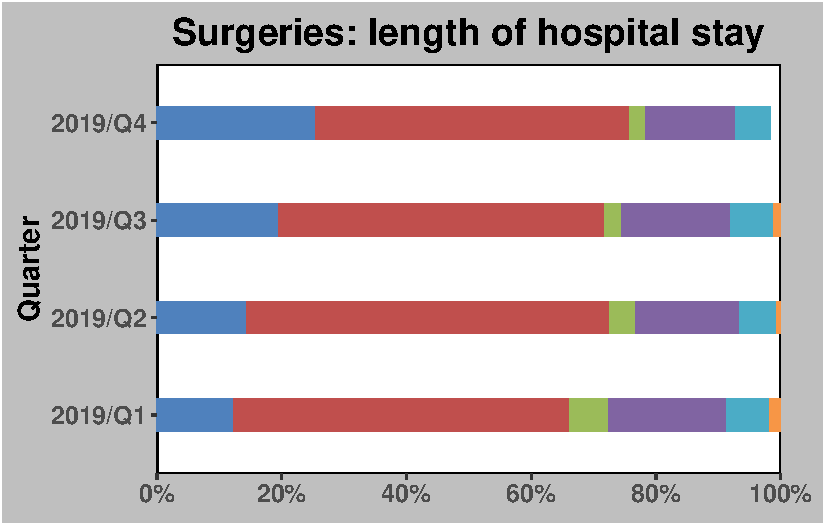
\includegraphics{graph_makeover_files/figure-pdf/unnamed-chunk-3-1.pdf}

}

\end{figure}

\hypertarget{making-assumptions}{%
\subsection{Making assumptions}\label{making-assumptions}}

When I look at this chart, before I even get into the specifics I first
have two key questions:

\begin{itemize}
\tightlist
\item
  Who is the audience for this graph?
\item
  What is the point of this graph?
\end{itemize}

Now, we have to make assumptions about the audience for the purpose of
this exercise: so let's assume this is designed to inform the executive
leadership team at a hospital.

Ok, but what are we trying to tell them using this graph? Well, the data
appears to be telling a success story: between Q1 and Q4 in 2019 the
proportion of patients who stayed more than 24 hours in hospital after
surgery decreased.

Notice that I'm making further assumptions here: I assume that the
categories are measuring hours, and I assume that what's being measured
is length of stay in hospital after surgery. In the absence of other
evidence, these seem like reasonable assumptions to make.

\hypertarget{making-it-better}{%
\subsection{Making it better}\label{making-it-better}}

To quote from the Storytelling With Data website:

\begin{quote}
Imagine the person who created this visual asks you for your opinion.
What feedback might you provide to improve its effectiveness? Consider
not only what you would change, but also why. What is the benefit of
incorporating your points of critique?
\end{quote}

So we have an assumed audience (ELT at the hospital), and we have a
narrative (in 2019 there was a quarter-on-quarter decline in
post-surgery lengths of stay at the hospital). How can we improve the
existing visual to communicate this point effectively to our assumed
audience?

\hypertarget{title}{%
\subsubsection{Title}\label{title}}

Let's start at the top: with the title of the chart. There are two
things that we can improve here: the position and content of that title.

What's wrong with the position? Well, many cultures around the world
read from left to right, and that's certainly true in the
English-speaking world.
\href{https://www.storytellingwithdata.com/blog/2012/09/quick-tip-left-uppermost-align-title}{Storytelling
With Data's very own Cole Knaflic} has written about the need to
left-align graph titles, and
\href{https://web.archive.org/web/20130310105837/http://styleguide.yahoo.com/writing/write-web/eye-tracking-where-do-readers-look-first}{research
elsewhere} backs this up: put your titles on the top left, as that's
where your audience will look first.

But why do we \emph{want} our audience to read the title first anyway?
It's simple: in just a few short words, your title will tell them
everything they need to know about the chart. Sometimes your audience
will either be too busy to scrutinise your graph, or else they may not
understand if even if they do. So think of your title as both a summary
and a guide: it gives the reader the information they need to make a
decsion (even if that decision is to ask for more data), \emph{and} it
gives them the information they need to understand what's in the graph
below. A good title is both self-sufficient and complementary.

We'll come back to the precise wording of this title once we've
deconstructed the visuals beneath it a little further.

\hypertarget{chart-type}{%
\subsubsection{Chart type}\label{chart-type}}

The original graph is presented in the form of stacked bar charts, with
time along the Y axis and the metric (share of post-operative patients)
along the X axis. The categories, which split the bars into their
coloured stacks, represent period of stay in hospital ranging from 24
hours or less to greater than or equal to 60 hours, with an additional
category for ``Unknown''.

There are two drawbacks with representing change over time in this way:
firstly, we have to read from bottom to top along the Y axis, and
secondly we have to determine the change over that time by comparing the
width of each segment in each row. This is a challenging exercise to
undertake, but we can ease the cognitive load on the reader by making
one simple adjustment: convert the stacked bar chart into a line chart.

\begin{Shaded}
\begin{Highlighting}[]
\FunctionTok{ggplot}\NormalTok{(}
  \AttributeTok{data =}\NormalTok{ hosital\_stay\_reshaped,}
  \FunctionTok{aes}\NormalTok{(}\AttributeTok{x =}\NormalTok{ position, }\AttributeTok{y =}\NormalTok{ value, }\AttributeTok{group =}\NormalTok{ name)}
\NormalTok{) }\SpecialCharTok{+}
  \FunctionTok{geom\_line}\NormalTok{() }\SpecialCharTok{+}
  \FunctionTok{geom\_point}\NormalTok{(}\AttributeTok{size=}\FloatTok{2.5}\NormalTok{) }\SpecialCharTok{+}
  \FunctionTok{scale\_x\_continuous}\NormalTok{(}\AttributeTok{limits =} \FunctionTok{c}\NormalTok{(}\DecValTok{1}\NormalTok{,}\FloatTok{4.3}\NormalTok{), }\AttributeTok{labels =} \FunctionTok{c}\NormalTok{(}\StringTok{"Q1"}\NormalTok{, }\StringTok{"Q2"}\NormalTok{, }\StringTok{"Q3"}\NormalTok{, }\StringTok{"Q4"}\NormalTok{)) }\SpecialCharTok{+}
  \FunctionTok{scale\_y\_continuous}\NormalTok{(}\AttributeTok{breaks =} \FunctionTok{c}\NormalTok{(}\DecValTok{0}\NormalTok{,.}\DecValTok{1}\NormalTok{,.}\DecValTok{2}\NormalTok{,.}\DecValTok{3}\NormalTok{,.}\DecValTok{4}\NormalTok{,.}\DecValTok{5}\NormalTok{,.}\DecValTok{6}\NormalTok{), }\AttributeTok{labels =}\NormalTok{ scales}\SpecialCharTok{::}\NormalTok{percent) }\SpecialCharTok{+}
\NormalTok{  purrr}\SpecialCharTok{::}\FunctionTok{map2}\NormalTok{(}
    \AttributeTok{.x =} \FunctionTok{c}\NormalTok{(}\FloatTok{0.017}\NormalTok{, }\FloatTok{0.027}\NormalTok{, }\FloatTok{0.056}\NormalTok{, }\FloatTok{0.144}\NormalTok{, }\FloatTok{0.254}\NormalTok{, }\FloatTok{0.503}\NormalTok{),}
    \AttributeTok{.y =} \FunctionTok{c}\NormalTok{(}\StringTok{"Unknown"}\NormalTok{, }\StringTok{"36 and 48"}\NormalTok{, }\StringTok{"\textgreater{}=60"}\NormalTok{, }\StringTok{"48 and 59"}\NormalTok{, }\StringTok{"\textless{}=24"}\NormalTok{, }\StringTok{"24 and 36"}\NormalTok{),}
    \AttributeTok{.f =} \SpecialCharTok{\textasciitilde{}}\FunctionTok{annotate}\NormalTok{(}\AttributeTok{geom =} \StringTok{"text"}\NormalTok{, }\AttributeTok{x =} \DecValTok{4}\NormalTok{, }\AttributeTok{y =}\NormalTok{ .x, }\AttributeTok{hjust=}\SpecialCharTok{{-}}\FloatTok{0.2}\NormalTok{, }\AttributeTok{size=}\FloatTok{5.5}\NormalTok{, }\AttributeTok{label =}\NormalTok{ .y)}
\NormalTok{  ) }\SpecialCharTok{+}
  \FunctionTok{labs}\NormalTok{(}
    \AttributeTok{title =} \StringTok{"Surgeries: length of hospital stay"}
\NormalTok{  ) }\SpecialCharTok{+}
  \FunctionTok{theme\_minimal}\NormalTok{() }\SpecialCharTok{+}
  \FunctionTok{theme}\NormalTok{(}
    \AttributeTok{axis.title =} \FunctionTok{element\_blank}\NormalTok{(),}
    \AttributeTok{plot.title.position =} \StringTok{"plot"}\NormalTok{,}
    \AttributeTok{panel.grid.major.x =} \FunctionTok{element\_blank}\NormalTok{(),}
    \AttributeTok{panel.grid.minor.x =} \FunctionTok{element\_blank}\NormalTok{(),}
    \AttributeTok{panel.grid.minor.y =} \FunctionTok{element\_blank}\NormalTok{(),}
    \AttributeTok{axis.text =} \FunctionTok{element\_text}\NormalTok{(}\AttributeTok{size=}\DecValTok{14}\NormalTok{),}
    \AttributeTok{plot.title =} \FunctionTok{element\_text}\NormalTok{(}\AttributeTok{size=}\DecValTok{18}\NormalTok{)}
\NormalTok{  )}
\end{Highlighting}
\end{Shaded}

\begin{figure}[H]

{\centering 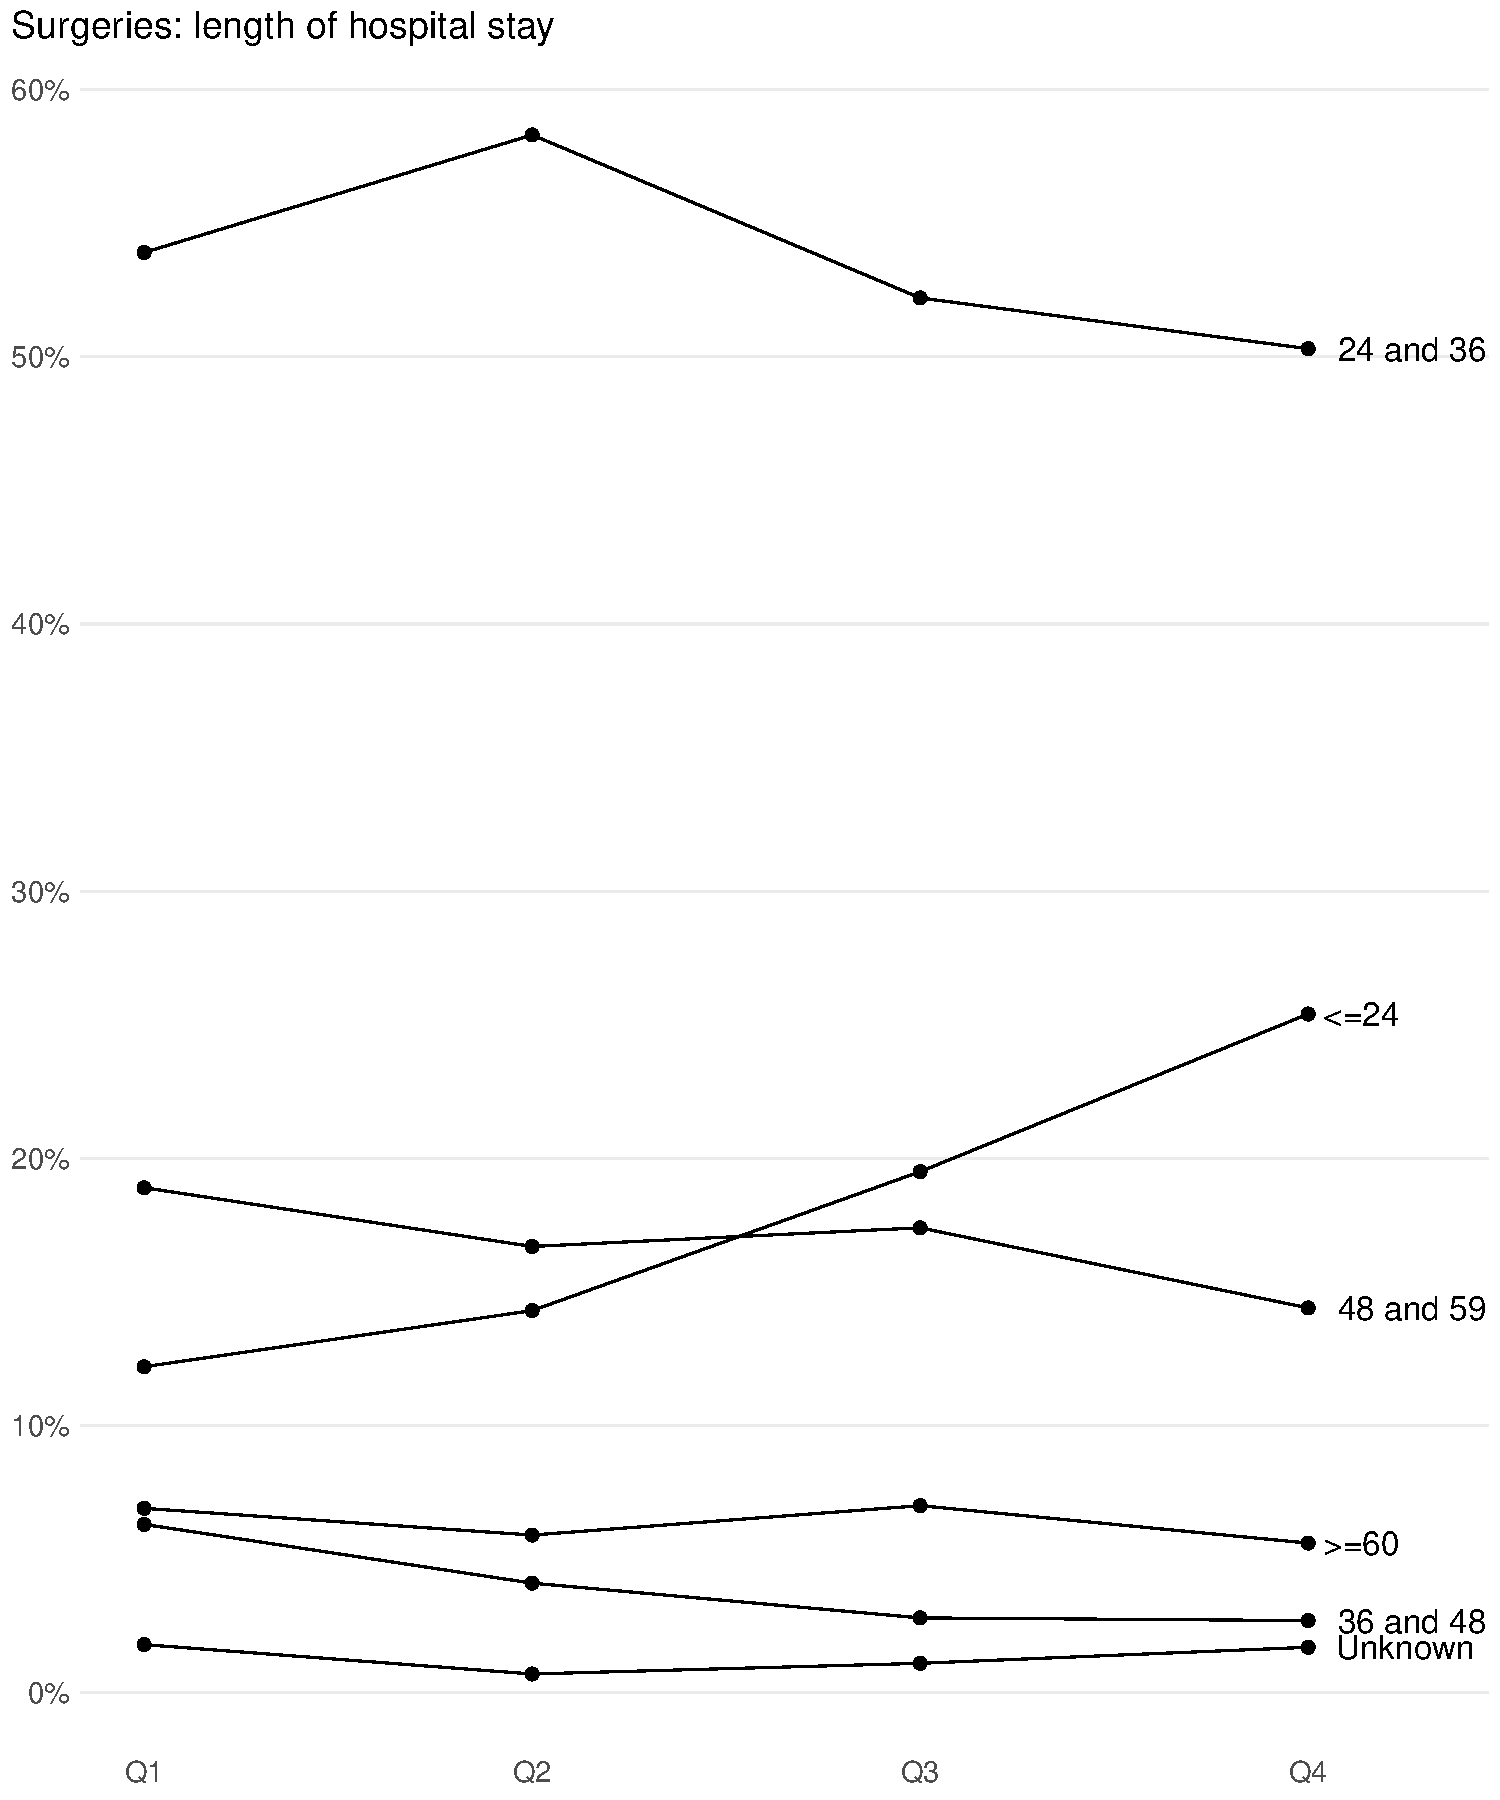
\includegraphics{graph_makeover_files/figure-pdf/unnamed-chunk-4-1.pdf}

}

\end{figure}

We can now see the change over time in each category more clearly, and
the rise in the ``\textless=24'' category stands out much more than it
did in the stacked bar chart.

Notice how I've also labelled the categories directly in the chart
rather than add a legend, which saves us space in the visual and makes
it easy for the reader to associate each line with its respective
category.

Because of my decision to label the lines directly, I was able to
completely remove the colours from this chart for the time being. This
is a useful thing to do as you iterate: make sure your chart works well
in black and white first before you start introducing colours. This
forces you to think carefully about how to use colour, layering colours
onto the graph as needed but still adhering to standards of
accessibility in your visual design.

Finally, I've kept other visual elements to a minimum: only horizontal
grid lines at each 10\% mark, and simplifying the X-axis labels to
``Q1'', ``Q2'' and so on. We'll clarify which year we're looking at
later when we re-examine the content of our title (which, as you've
probably noticed, is now left-aligned).

\hypertarget{title-reprise}{%
\subsubsection{Title Reprise}\label{title-reprise}}

Now that we've visualised the data in a way that makes the message a
little clearer, let's look again at the content of our title.

The current title refers to ``length of hospital stay'', but what we're
visualising is the proportion of post-operative patients who stay in
hospital for varying lengths of time. Let's spell this out in our title
as so:

\begin{quote}
The share of patients who stayed in hospital after surgery by length of
stay
\end{quote}

This is ok I guess, but it's still a bit confusing. More importantly, it
says little about the \emph{point} of this graph: what am I looking at
here? Why should I care?

Let's try again:

\begin{quote}
In 2019, the share of patients who stayed in hospital for less than 24
hours after surgey increased between Q1 and Q4
\end{quote}

This is better: not only is this title telling us the key point, it's
also telling us that we're looking at data about 2019 here (a detail we
decided to remove from the graph). We could reflect on this title
further and make further improvements, but let's move on for now and
take another look at the graph.

\hypertarget{emphasise-the-point}{%
\subsubsection{Emphasise the Point}\label{emphasise-the-point}}

We now have a chart that makes sense for what we're trying to say about
our data, and we've written a title that tells the audience what they
need to know. This is already an improvement on what we started with,
but we can do better: we need to draw the reader's attention to what's
important in the graph, and de-emphasise what's less important.

Here's one way of achieving this:

\begin{Shaded}
\begin{Highlighting}[]
\FunctionTok{ggplot}\NormalTok{(}
  \AttributeTok{data =}\NormalTok{ hosital\_stay\_reshaped,}
  \FunctionTok{aes}\NormalTok{(}\AttributeTok{x =}\NormalTok{ position, }\AttributeTok{y =}\NormalTok{ value, }\AttributeTok{group =}\NormalTok{ name)}
\NormalTok{) }\SpecialCharTok{+}
  \FunctionTok{geom\_line}\NormalTok{(}\FunctionTok{aes}\NormalTok{(}\AttributeTok{colour =}\NormalTok{ emphasis), }\AttributeTok{size =} \FloatTok{2.5}\NormalTok{) }\SpecialCharTok{+}
  \FunctionTok{geom\_point}\NormalTok{(}\AttributeTok{size=}\FloatTok{2.5}\NormalTok{) }\SpecialCharTok{+}
  \FunctionTok{scale\_x\_continuous}\NormalTok{(}\AttributeTok{limits =} \FunctionTok{c}\NormalTok{(}\DecValTok{1}\NormalTok{,}\FloatTok{4.3}\NormalTok{), }\AttributeTok{labels =} \FunctionTok{c}\NormalTok{(}\StringTok{"Q1"}\NormalTok{, }\StringTok{"Q2"}\NormalTok{, }\StringTok{"Q3"}\NormalTok{, }\StringTok{"Q4"}\NormalTok{)) }\SpecialCharTok{+}
  \FunctionTok{scale\_y\_continuous}\NormalTok{(}\AttributeTok{breaks =} \FunctionTok{c}\NormalTok{(}\DecValTok{0}\NormalTok{,.}\DecValTok{1}\NormalTok{,.}\DecValTok{2}\NormalTok{,.}\DecValTok{3}\NormalTok{,.}\DecValTok{4}\NormalTok{,.}\DecValTok{5}\NormalTok{,.}\DecValTok{6}\NormalTok{), }\AttributeTok{labels =}\NormalTok{ scales}\SpecialCharTok{::}\NormalTok{percent) }\SpecialCharTok{+}
  \FunctionTok{scale\_colour\_manual}\NormalTok{(}\AttributeTok{values =} \FunctionTok{c}\NormalTok{(}\StringTok{"\#d9ded6"}\NormalTok{, }\StringTok{"\#f3a144"}\NormalTok{)) }\SpecialCharTok{+}
\NormalTok{  purrr}\SpecialCharTok{::}\FunctionTok{map2}\NormalTok{(}
    \AttributeTok{.x =} \FunctionTok{c}\NormalTok{(}\FloatTok{0.017}\NormalTok{, }\FloatTok{0.027}\NormalTok{, }\FloatTok{0.056}\NormalTok{, }\FloatTok{0.144}\NormalTok{, }\FloatTok{0.254}\NormalTok{, }\FloatTok{0.503}\NormalTok{),}
    \AttributeTok{.y =} \FunctionTok{c}\NormalTok{(}\StringTok{"Unknown"}\NormalTok{, }\StringTok{"36 and 48"}\NormalTok{, }\StringTok{"\textgreater{}=60"}\NormalTok{, }\StringTok{"48 and 59"}\NormalTok{, }\StringTok{"\textless{}=24"}\NormalTok{, }\StringTok{"24 and 36"}\NormalTok{),}
    \AttributeTok{.f =} \SpecialCharTok{\textasciitilde{}}\FunctionTok{annotate}\NormalTok{(}\AttributeTok{geom =} \StringTok{"text"}\NormalTok{, }\AttributeTok{x =} \DecValTok{4}\NormalTok{, }\AttributeTok{y =}\NormalTok{ .x, }\AttributeTok{hjust=}\SpecialCharTok{{-}}\FloatTok{0.2}\NormalTok{, }\AttributeTok{size=}\FloatTok{5.5}\NormalTok{, }\AttributeTok{label =}\NormalTok{ .y)}
\NormalTok{  ) }\SpecialCharTok{+}
  \FunctionTok{labs}\NormalTok{(}
    \AttributeTok{title =} \StringTok{"In 2019, the share of patients who stayed in hospital for \textless{}span style=\textquotesingle{}color:\#f3a144\textquotesingle{}\textgreater{}less than\textless{}br\textgreater{}24 hours\textless{}/span\textgreater{} after surgey increased between Q1 and Q4"}
\NormalTok{  ) }\SpecialCharTok{+}
  \FunctionTok{theme\_minimal}\NormalTok{() }\SpecialCharTok{+}
  \FunctionTok{theme}\NormalTok{(}
    \AttributeTok{axis.title =} \FunctionTok{element\_blank}\NormalTok{(),}
    \AttributeTok{legend.position =} \StringTok{"none"}\NormalTok{,}
    \AttributeTok{plot.title.position =} \StringTok{"plot"}\NormalTok{,}
    \AttributeTok{plot.title =} \FunctionTok{element\_markdown}\NormalTok{(}\AttributeTok{size=}\DecValTok{24}\NormalTok{),}
    \AttributeTok{panel.grid.major.x =} \FunctionTok{element\_blank}\NormalTok{(),}
    \AttributeTok{panel.grid.minor.x =} \FunctionTok{element\_blank}\NormalTok{(),}
    \AttributeTok{panel.grid.minor.y =} \FunctionTok{element\_blank}\NormalTok{(),}
    \AttributeTok{axis.text =} \FunctionTok{element\_text}\NormalTok{(}\AttributeTok{size=}\DecValTok{12}\NormalTok{)}
\NormalTok{  )}
\end{Highlighting}
\end{Shaded}

\begin{figure}[H]

{\centering 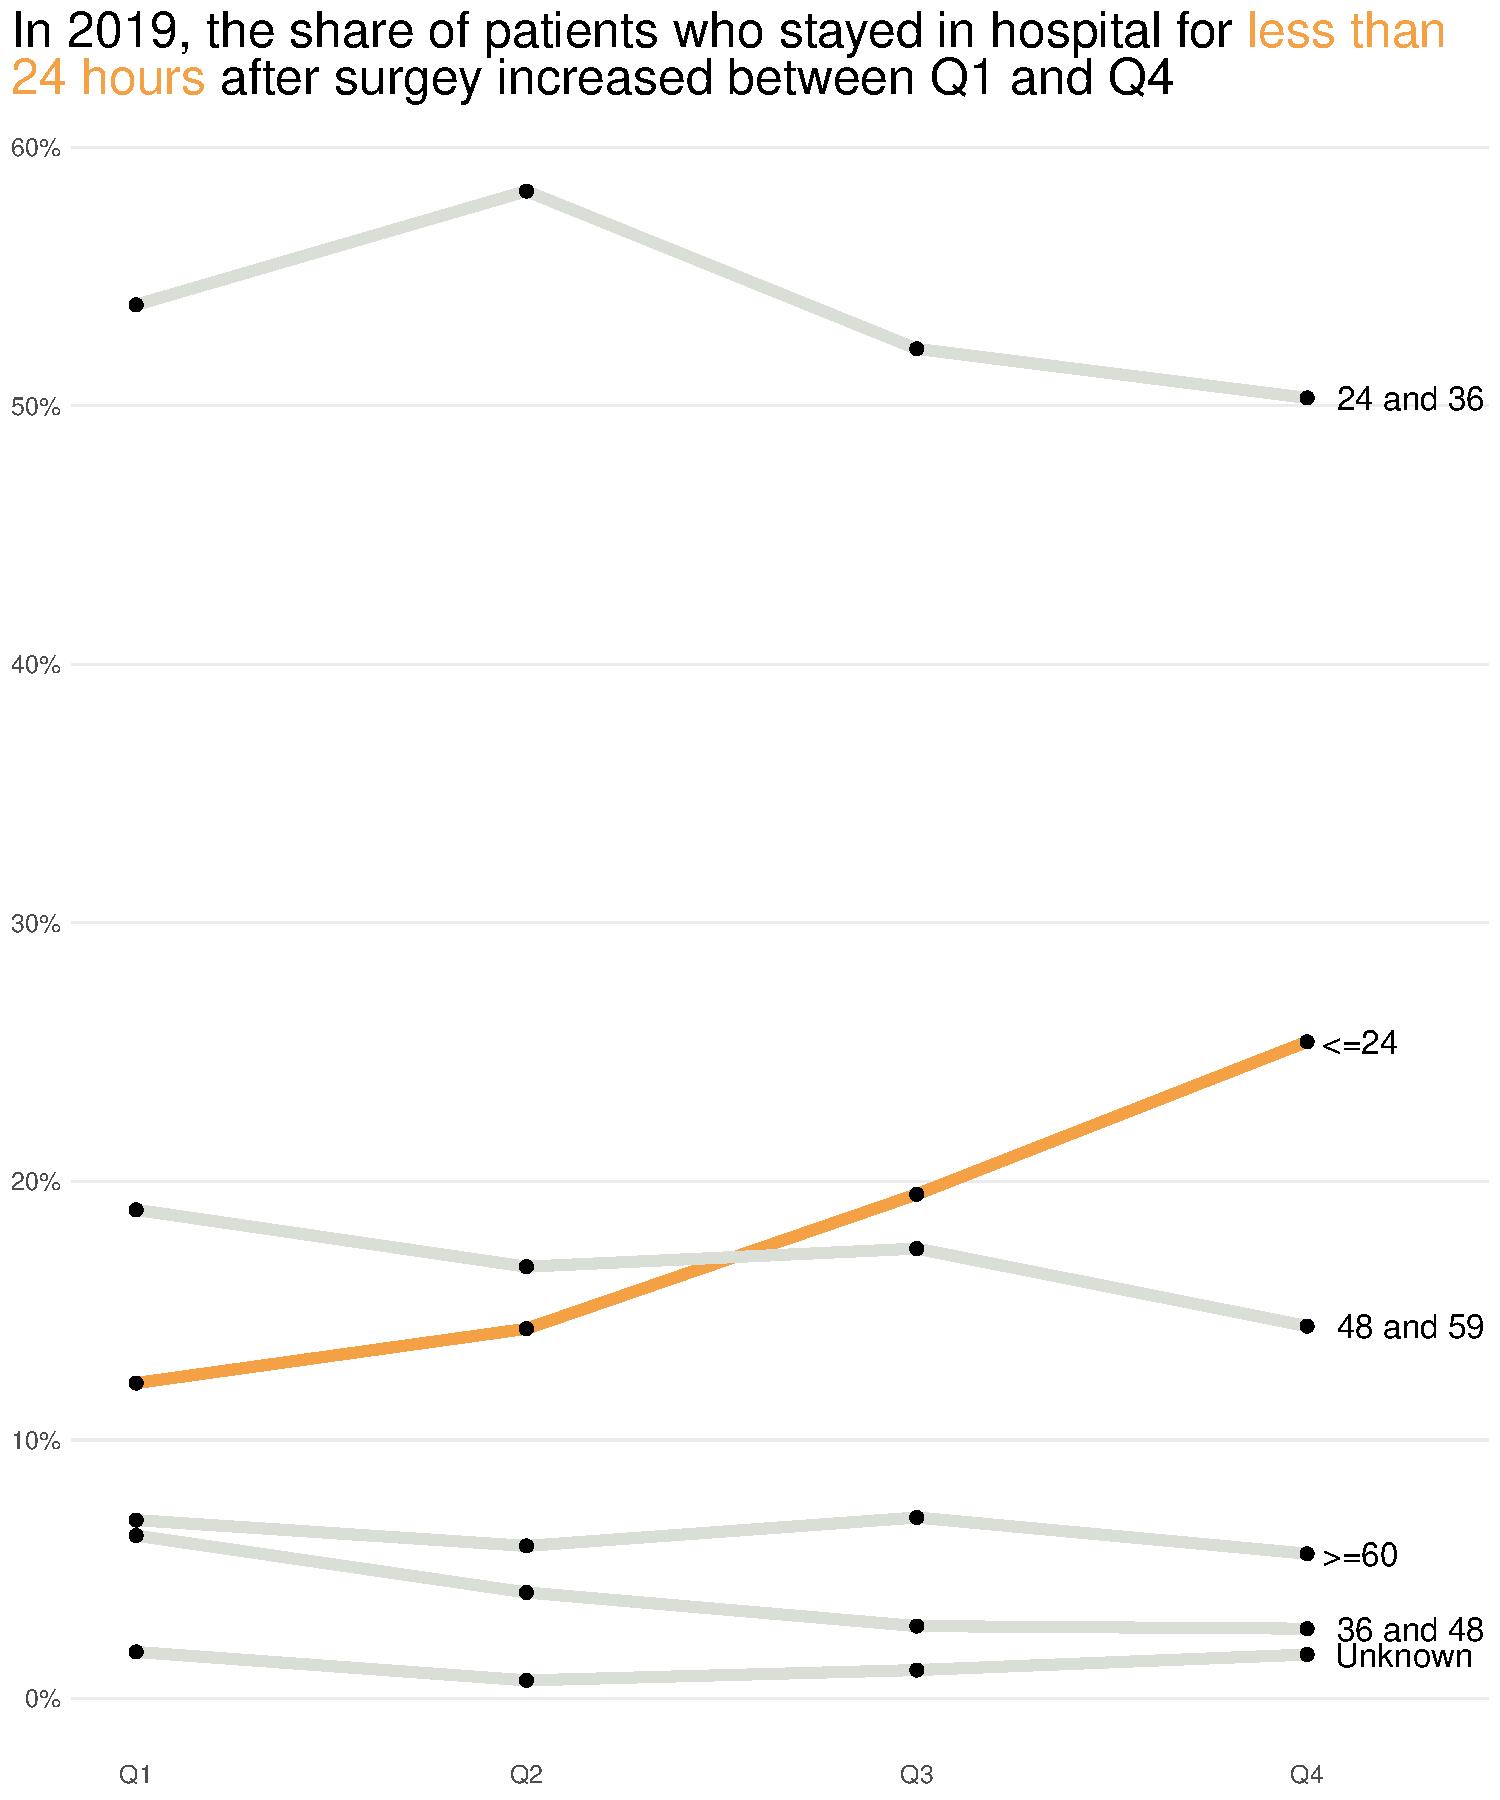
\includegraphics{graph_makeover_files/figure-pdf/unnamed-chunk-5-1.pdf}

}

\end{figure}

By thoughtfully introducing some colour into our graph, we've drawn
attention to the line that matters (``\textless=24'') by highlighting it
in orange. We've simultaneously de-emphasises the lines that matter less
by making them grey; they're still there, but that's not where the
reader's attention is drawn. As an added touch, we've added the same
orange colour to some of the text in our title: this instantly creates
the necessary association between a detail in the title and a detail in
the visual.

\hypertarget{boiling-it-right-down}{%
\subsubsection{Boiling It Right Down}\label{boiling-it-right-down}}

We've



\end{document}
